
\subsection{Question Group 2 - Blockchain Knowledge and Opinions}

This section features some questions that inquire about the respondent's knowledge in blockchain, and their opinions about the relationship between cryptocurrencies and blockchain. Are blockchains independent of cryptocurrencies or not? And in which cases? These are questions that will also help decide the need of a cryptocurrency for the design of the system that was proposed.

\subsection*{1 - General Blockchain Knowledge.}
 %GRAFICO BLOCKCHAIN KNOWLEDGE
 \begin{figure}[h]
\centering
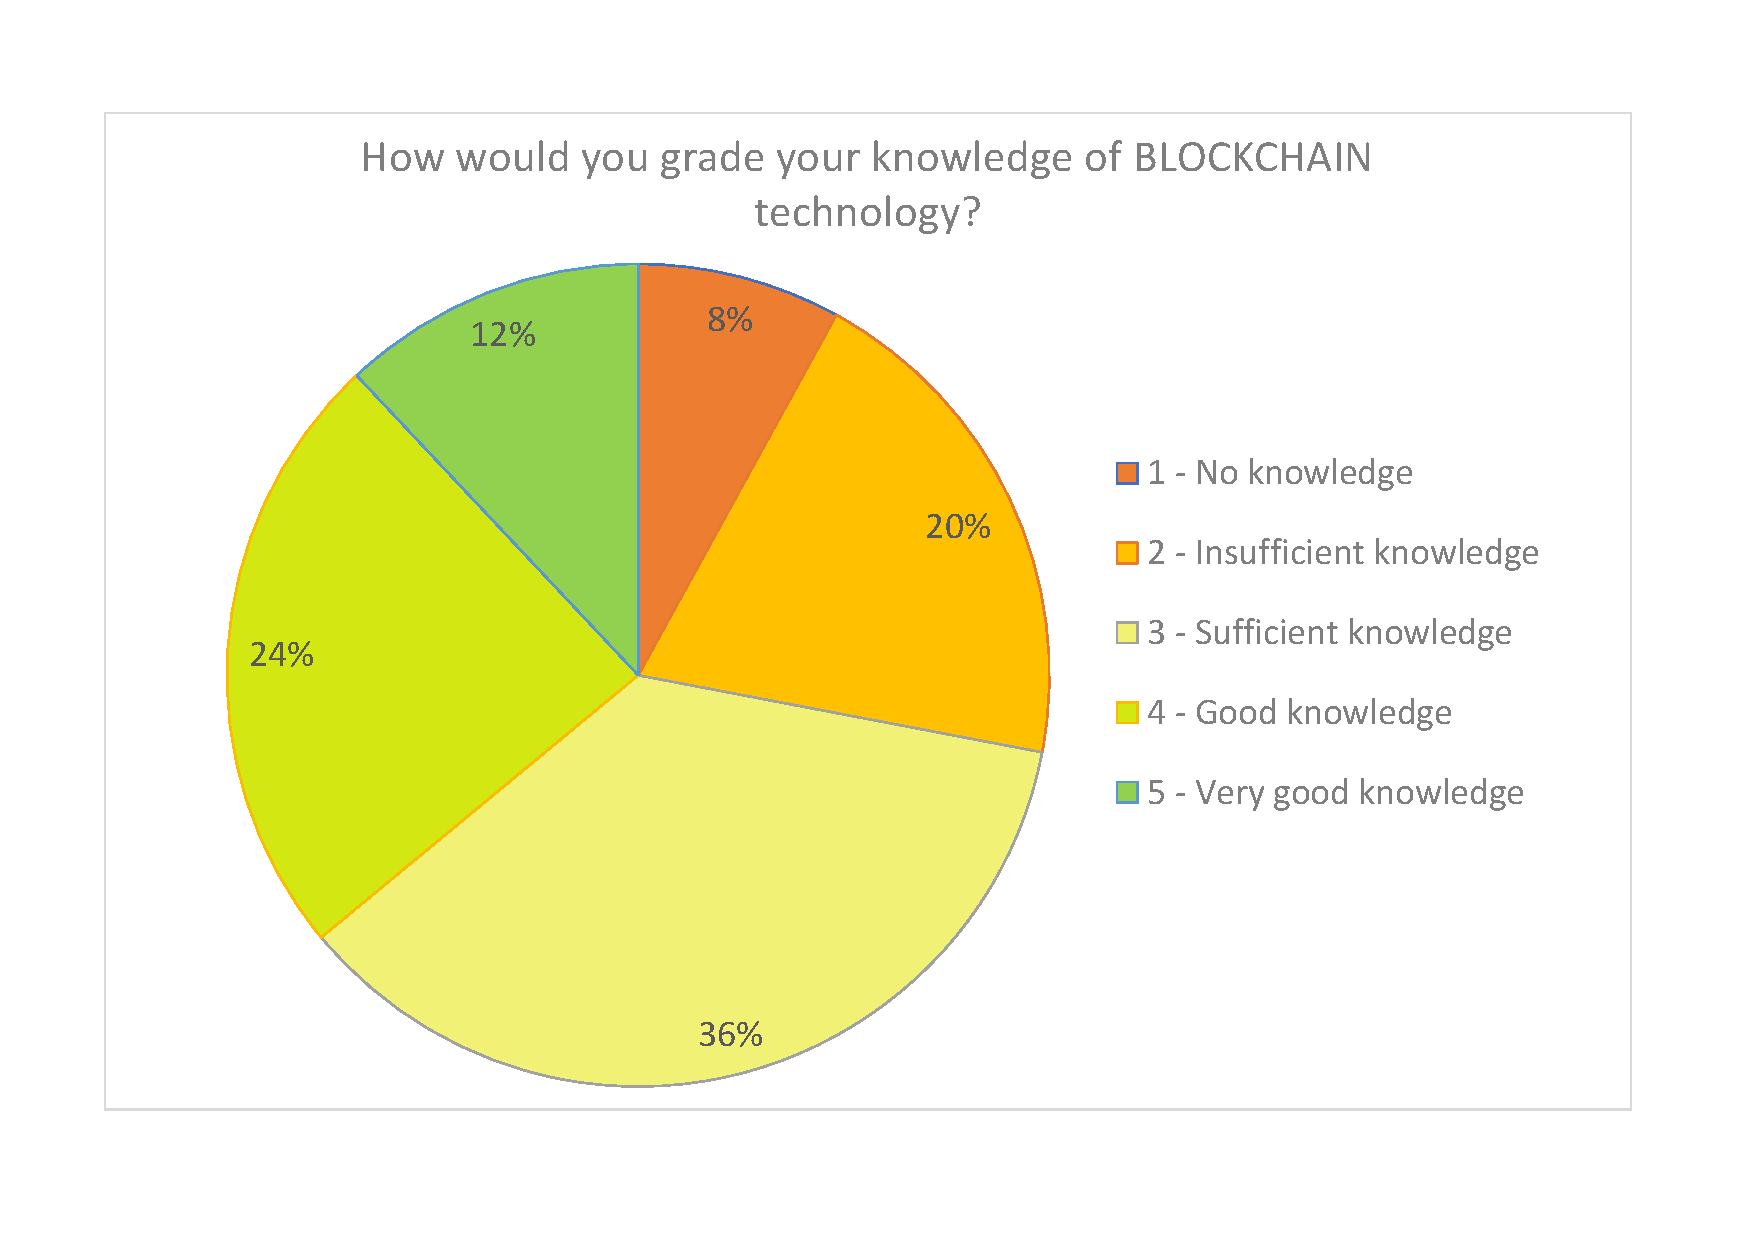
\includegraphics[scale=0.65]{media/survey_group2/blockchain_knowledge.pdf}
\caption{Question about Blockchain knowledge.}
\label{fig:blockchain_knowledge}
\end{figure}

In Figure~\ref{fig:blockchain_knowledge}, it can be seen that most answers are in the middle of the scale, while both the extremes have few answers, which closely resemble a gaussian or normal distribution. 

Indeed, when calculated, the skew of this data is about -0,065104294, which is a very low number (the standard error was about 0,46) and close to 0. A normal distribution has a skew of 0, so this can be said to be a good approximation. Additional, it can be said that there is not much of a bias towards accepting or denying blockchain when answering other questions, either from knowing too much or too little, since the knowledge curve seems to be normal.
 
\subsection*{2 - Rate the affirmations about the use of cryptocurrencies in the blockchain.}

After inquiring about the blockchain knowledge of the respondents, some affirmations were made about cryptocurrencies, which can be seen below. The question was optional, since respondents without sufficient knowledge of blockchain might face difficulties understanding the affirmations.


%GRAFICOS DE CADA 1 DAS 3 AFIRMAÇÕES DE CRYPTOCURRENCIES
\textbf{Affirmations: }
\begin{enumerate}
\item A blockchain always needs to have a cryptocurrency attached in order to work well.
\item Cryptocurrencies are useful in blockchains open to the public, in order to create incentives for good behavior, but not always necessary in private chains.
\item Blockchains can be useful in some uses cases, independently of whether they hold a cryptocurrency or not.
\end{enumerate}

Independently, these affirmations do not hold an absolute value that can help ascertain if there is a need for a cryptocurrency in the case of supply chain. But together, the three affirmations lead to a higher degree of certainty.

The first affirmation states that a blockchain, any at all, independently of the purpose or type, does indeed need a cryptocurrency. The second affirmation goes on a tangent from the first one, stating that maybe cryptocurrencies are only needed as an incentive, and otherwise could be not needed. The final affirmation is more generic in nature, and attempts to \textbf{completely separate the concept of blockchain and cryptocurrency}. The results for each affirmation can be found in Figure~\ref{fig:blockchain_crypto_opinions} and in Table~\ref{table:blockchain_crypto_opinions}.

\begin{figure}[h]
\centering
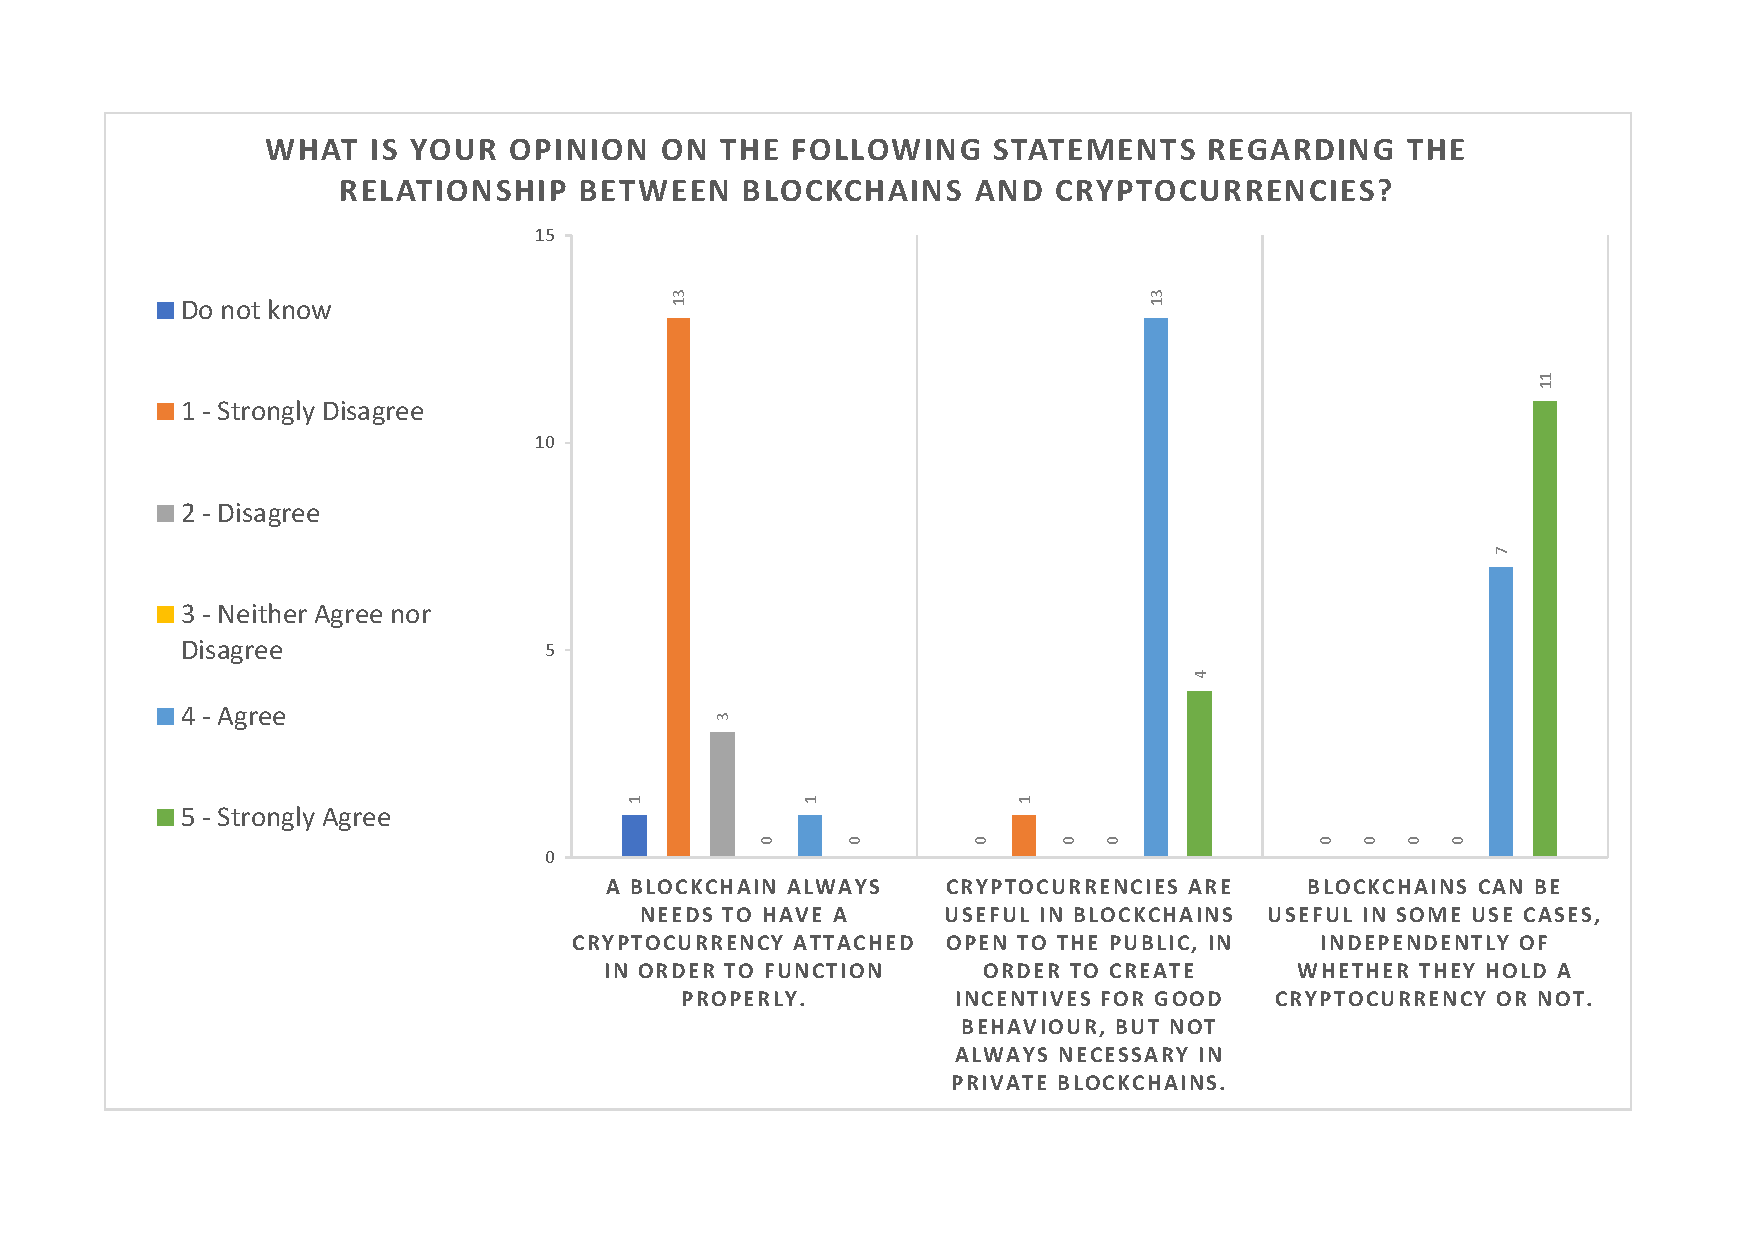
\includegraphics[scale=0.95]{media/survey_group2/blockchain_crypto_opinions.pdf}
\caption{Question to rate affirmations about the use of cryptocurrencies in the blockchain.}
\label{fig:blockchain_crypto_opinions}
\end{figure}



%%%%%% TABLE START %%%%%%%%%%%%%%
% Please add the following required packages to your document preamble:
% \usepackage[normalem]{ulem}
% \useunder{\uline}{\ul}{}
\begin{table}[ht]
    \centering
    \caption{Question results metrics for the affirmations about the use of cryptocurrencies in the blockchain.}
    \label{table:blockchain_crypto_opinions}
    \resizebox{\textwidth}{!}{
    \begin{tabular}{l|c|c|c|c|c|c|}
    \cline{2-7}
                                                                                                                                                                & \multicolumn{1}{l|}{Mode} & \multicolumn{1}{l|}{Median} & \multicolumn{1}{l|}{Mean} & \multicolumn{1}{l|}{\begin{tabular}[c]{@{}l@{}}Standard\\  Deviation\end{tabular}} & \multicolumn{1}{l|}{Range} & \multicolumn{1}{l|}{Skewness} \\ \hline
    \multicolumn{1}{|l|}{\begin{tabular}[c]{@{}l@{}}1. Blockchain needs \\ cryptocurrencies to work well\end{tabular}}                                          & 1                         & 1                           & 1,36                      & 0,79                                                                               & 3                          & 2,74                          \\ \hline
    \multicolumn{1}{|l|}{\begin{tabular}[c]{@{}l@{}}2.  Cryptocurrencies are only \\ useful as incentives in public \\ blockchains\end{tabular}}                & 4                         & 4                           & 4,06                      & 0,87                                                                               & 4                          & -2,51                         \\ \hline
    \multicolumn{1}{|l|}{\begin{tabular}[c]{@{}l@{}}3. Blockchains can be useful in\\ some cases, regardless of having \\ or not cryptocurrencies\end{tabular}} & 5                         & 5                           & 4,61                      & 0,50                                                                               & 1                          & -0,50                         \\ \hline
    \end{tabular}
    }
    \end{table}
%%%%%%%%%%% TABLE END %%%%%%%%%%%%%%%%%%%%%%%%%%%

\begin{itemize}
    \item The first affirmation has a very low agreement rate. Almost all of the respondents answered that they strongly disagreed with it, which can be seen in the table, as both the mode and median are 1, and the mean is also close to it. It can be concluded that, according to these opinions, \textbf{blockchain can sometimes not have a cryptocurrency and still perform well}.
    \item The second affirmation has a high agreement rate, with an average of 4.06. The mode and mean are also very close to the mean, and the standard deviation is lower than 1, which means that there is a consensus on the responses. Therefore, it can be concluded that, as per the opinions of the professionals, \textbf{a cryptocurrency is more useful in public blockchain contexts and applications, as an incentive, than in private blockchains, where these incentives are not needed.}
    \item The last affirmation has a very high agreement rate, the highest of them, with a mode and median of 5, and a mean of 4.61. There is a strong consensus, as all of the respondents answered with either 4 or 5 (Agree or Strongly Agree), leading to a low standard deviation and range. There is a slight skew, since the answers are distributed between these 2 items, with a bigger number of responses  on item 5. The conclusion for this affirmation is that \textbf{blockchains are useful, independently of holding a cryptocurrency or not}.
\end{itemize}


\subsection*{Conclusions from Question Group 2}

With these conclusions in mind, one final conclusion can be derived. If blockchains do not need cryptocurrencies to perform well (concluded from the non agreement with affirmation 1) and can generally still be useful without them (affirmation 3), then \textbf{cryptocurrencies should not be considered a necessity, but rather a design option, depending on the benefits} it can bring to a particular use case. Taking this conclusion into account, and also according to the agreement with affirmation 2, then: \textbf{if a blockchain design features a private blockchain, it does not necessarily need a cryptocurrency as a requirement, since incentives are not needed}. This is an especially interesting conclusion for the proof of concept.

%\subsection*{3 - Blockchain adoption challenges - maybe this one isnt that important to show}
% MAYBE TAKE THIS ONE OUT - NOT THAT IMPORTANT
